\documentclass{article}

\usepackage{url} 
\usepackage{geometry,afterpage}
\usepackage{pdfpages}
\usepackage{lastpage}
\usepackage{fancyhdr}
\usepackage{ngerman}
\usepackage{listings}

\usepackage{floatrow}
\usepackage[tableposition=top]{caption}
\floatsetup[table]{capposition=top}

\usepackage{amsmath, amssymb}

\usepackage[utf8]{inputenc}


\usepackage[numbib]{tocbibind}



\newcommand\twodigits[1]{%
   \ifnum#1<10 0#1\else #1\fi
}



\lhead{Bandabstand Germanium}
\rhead{21.05.2021\\ J. Winkler}
%\cfoot{\twodigits{\thepage}~/ \pageref{LastPage}}
\cfoot{{\thepage}~/ \pageref{LastPage}}


\newcommand{\Ekin}{E_\text{kin}}

\begin{document}

\parindent0cm


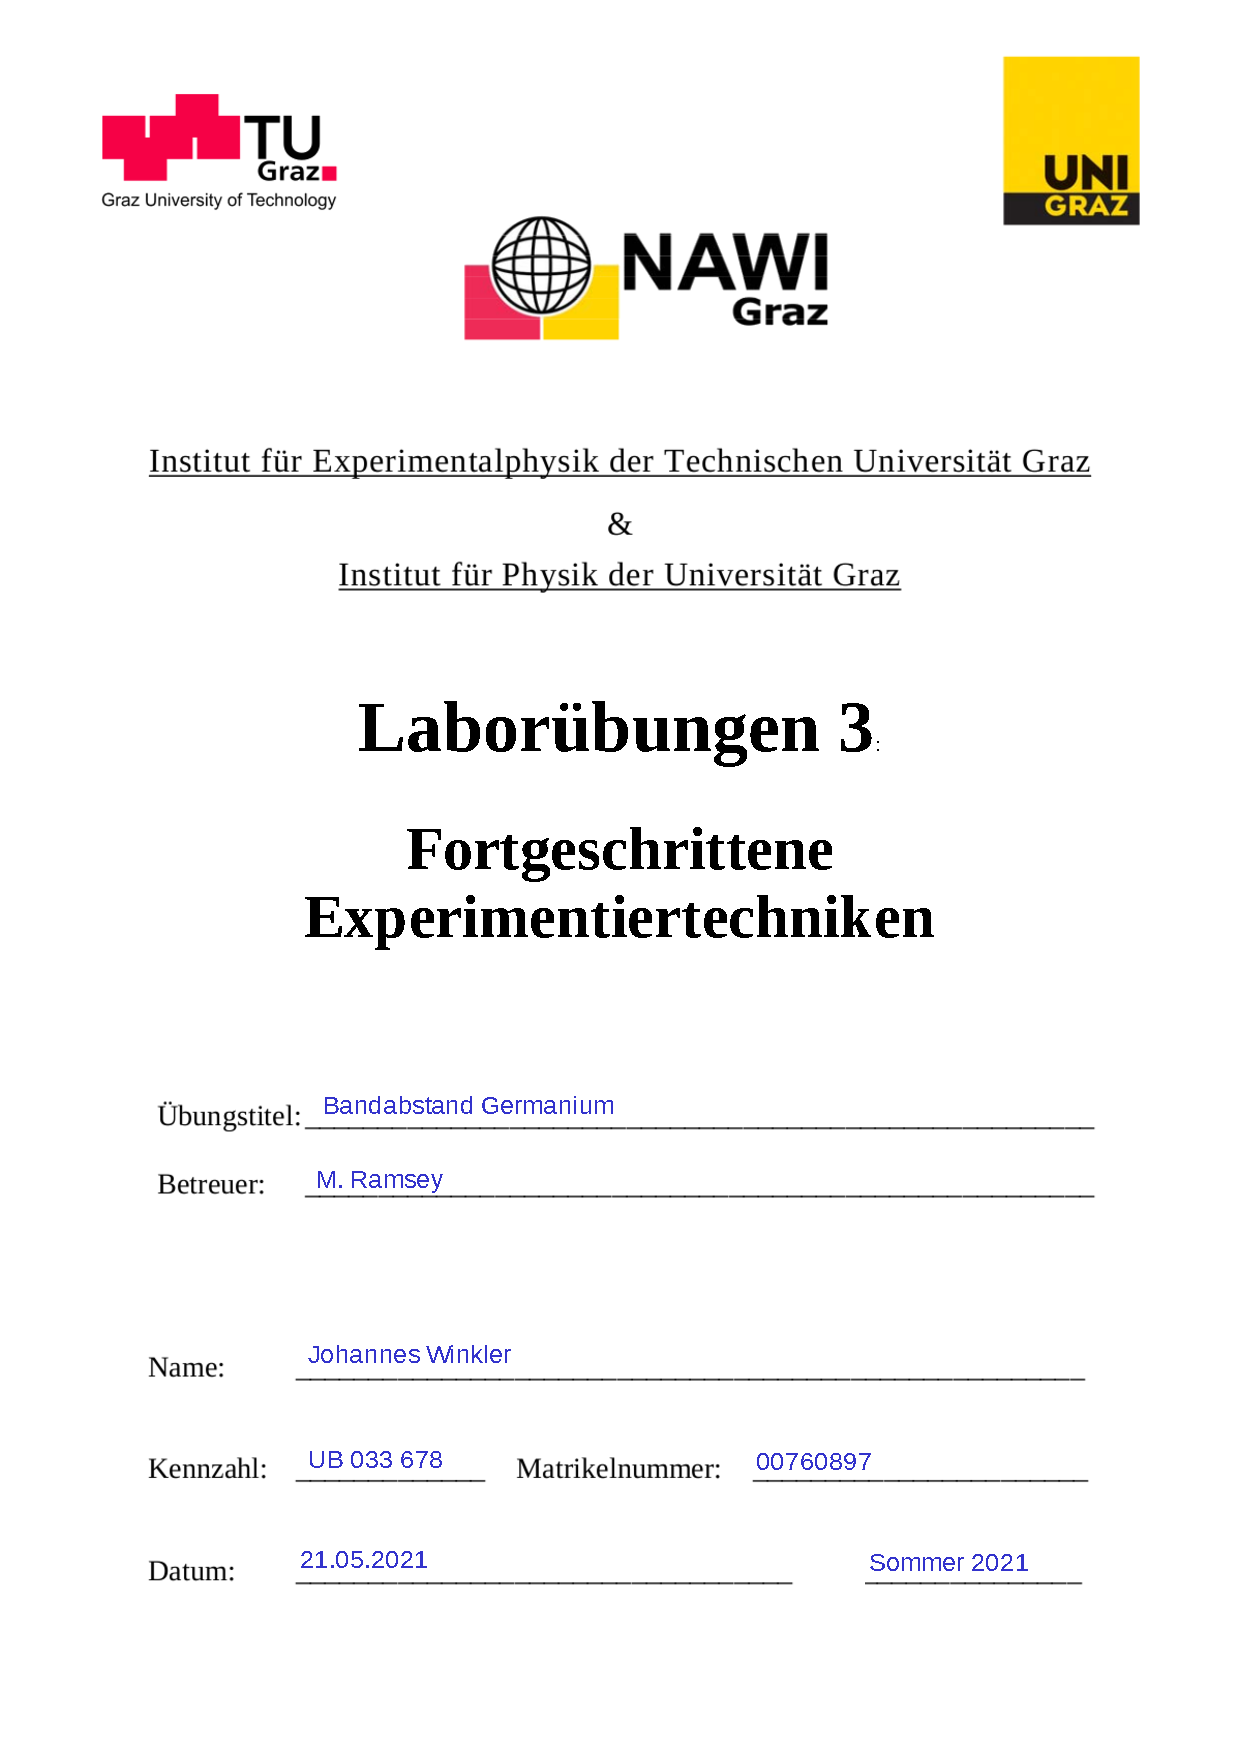
\includepdf{Deckblatt_neu_custom.pdf}

\tableofcontents
\newpage

\pagestyle{fancy}

\section{Aufgabenstellung}

\begin{enumerate}
\item Messung des Spannungsabfalls an einem undotierten Ge-Kristall bei
konstantem Strom durch den Kristall in Abhängigkeit von der Temperatur und
Berechnung der Leitfähigkeit $\sigma$ bzw. des spezifischen Widerstandes $\rho$.
\item Bestimmung des Bandabstandes $E_g$ von Germanium.
\item Messung des Spannungsabfalls analog zu Punkt 1 auch für einen p- oder n- dotierten Ge-Kristall
\end{enumerate}


%\begin{figure}[H]
%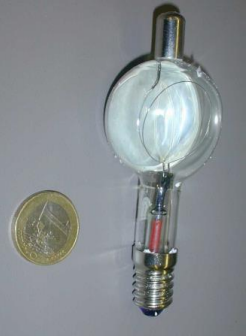
\includegraphics[scale=1.4]{versuch3.png}
%\caption{Vakuum Photozelle. Quelle: \cite{moodle}}
%\end{figure}

\section{Grundlagen}



\subsection{Halbleiter}
Halbleiter sind Stoffe, deren Leitfähigkeit von der Temperatur abhängig ist. Durch eine höhere Temperatur können die Elektronen im Valenzband dazu angeregt werden, ins Leiterband zu springen. Dadurch entsteht eine Leitfähigkeit. Halbleiter sind daher Heißleiter. Im Gegensatz dazu wird die Leitfähigkeit bei Metallen mit hoher Temperatur vermindert (Kaltleiter).

\subsection{Dotierung}
Halbleiter haben eine gewisse Eigenleitung (intrinsische Leitung). Diese ist allerdings relativ schwach. Durch Hinzugabe von Fremdatomen steigt die Leitfähigkeit an. Es können positive Ionen in den Halbleiter eingefügt werden (p-Dotierung) oder auch negative (n-Dotierung). Durch eine Dotierung erreicht man entweder einen Überschuss an Elektronen oder an Löchern. Grafisch veranschaulicht ist das in Abbildung~\ref{fig:bandabstand}.


\begin{figure}[H]
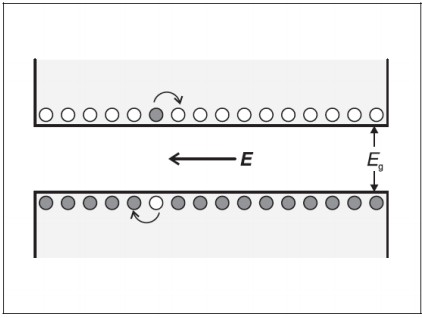
\includegraphics[scale=1.4]{bandabstand.png}
\caption{Veranschaulichung des Bändermodells. Quelle: \cite{moodle}}
\label{fig:bandabstand}
\end{figure}

\subsection{Formeln zur Berechnung}

Es wird ein Querstrom von $I_Q = 3~$mA angenommen. Aus Moodle ergibt sich die Formel zur Umrechnung von der Spannung UB zur Leitfähigkeit
\begin{align}
\sigma = \frac{I_Q [\text{mA}]}{\text{UB}~[\text{V}]}\cdot \frac{20~\text{mm}}{10\cdot\text{mm}\cdot 1~\text{mm}}
\label{eq:sigma}
\end{align} 
Die Umrechnung zwischen Temperatur und der Spannung UA ergibt sich laut \cite{moodle} aus
\begin{align}
T = 100~\text{K}\cdot \text{UA}~[\text{V}] + 237.15~\text{K}
\label{eq:T}
\end{align}
Es ergibt sich klarerweise, dass $\rho = 1/\sigma$.


\section{Versuchsaufbau}

\begin{figure}[H]
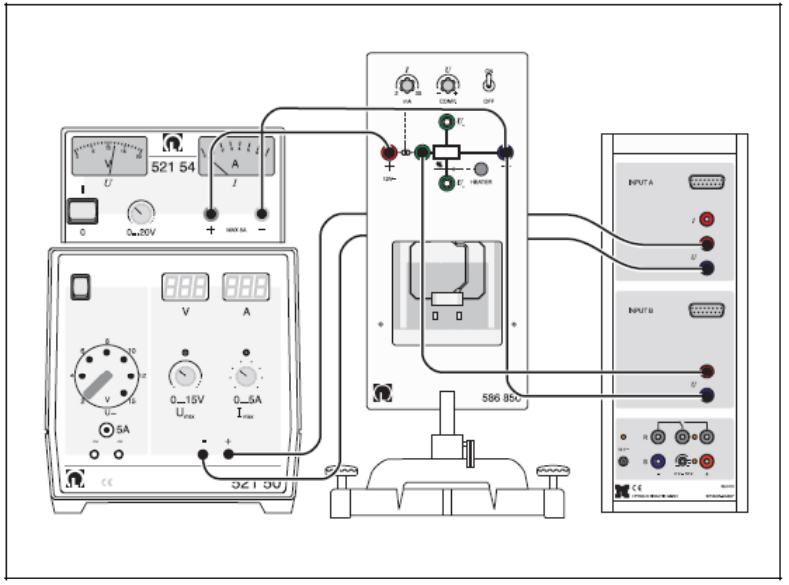
\includegraphics[scale=1.79]{versuchsaufbau.png}
\caption{Aufbau des Versuchs. Quelle: \cite{moodle}}
\label{fig:aufbau}
\end{figure}



\section{Geräteliste}


\begin{table}[H]
\caption{Liste der verwendeten Geräte}
~
\begin{tabular}{l|l}
 & Geräte  \\
\hline
1 & Versuchsapparatur für Hall-Effekt \\
2 & Cassy Sensor \\
3 & Computer mit Cassy-Lab 2 \\
4 & Germaniumkristall undotiert \\
5 & Germaniumkristall n-dotiert \\
6 & Germaniumkristall p-dotiert 
\end{tabular}

\end{table}

\newpage

\section{Durchführung und Messergebnisse}

Der Cassy Sensor wird per serieller Schnittstelle am Computer angeschlossen. Der Aufbau erfolgt gemäß Grafik~\ref{fig:aufbau}. Dann wird der Germaniumkristall aufgeheizt und regelmäßig die Temperatur und die Leitfähigkeit bestimmt. Die Temperatur ist linear abhängig von der Spannung UA. Die Leitfähigkeit bei konstantem Querstrom $I_Q=3~$mA ist indirekt proportional zur Spannung UB. Wie in \cite{moodle} beschrieben, werden diese beiden Spannungen alle 2 Sekunden gemessen. In den Grafiken~\ref{fig:data_raw} und~\ref{fig:data_scaled} werden die gemessenen Werte für die Spannungen gezeigt.



\begin{figure}[H]
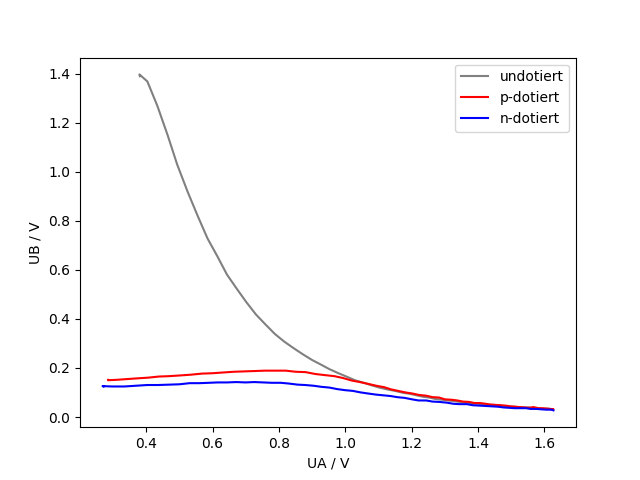
\includegraphics[scale=1.]{data_raw.png}
\caption{Spannungen wie sie gemessen wurden, wobei UA auf der x-Achse und UB1 auf der y-Achse aufgetragen wird.}
\label{fig:data_raw}
\end{figure}


\begin{figure}[H]
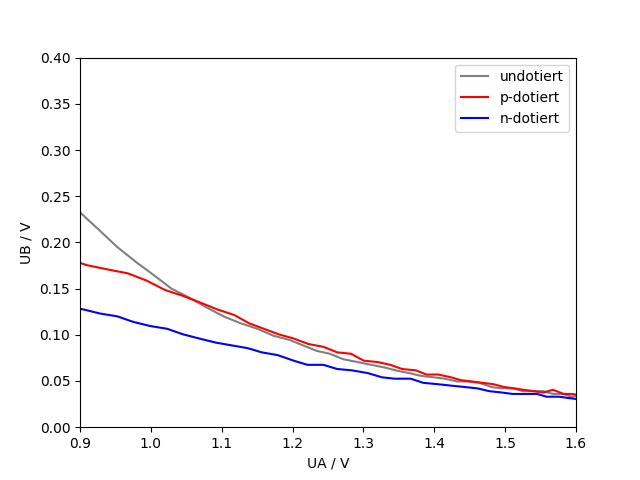
\includegraphics[scale=1.]{data_scaled.png}
\caption{Dieselben Spannungen wie Grafik~\ref{fig:data_raw}, mit eingeschränktem Wertebereich.}
\label{fig:data_scaled}
\end{figure}



\section{Auswertung}

Nach den Formeln~\eqref{eq:sigma} und \eqref{eq:T} können nun die Spannungen UA und UB in Temperatur und Leitfähigkeit umgerechnet werden. Dadurch kann Grafik~\ref{fig:data_raw} in transformierter Form angegeben werden.

\begin{figure}[H]
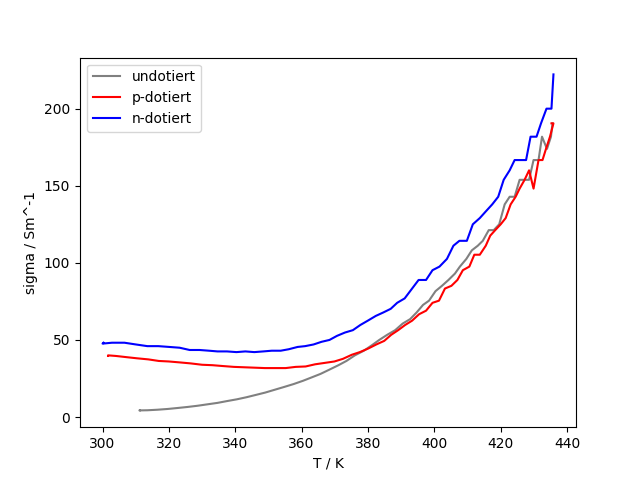
\includegraphics[scale=1.]{leitfaehigkeit.png}
\caption{Leitfähigkeit der Germanium-Kristalle abhängig von deren Temperatur.}
\label{fig:leitfaehigkeit}
\end{figure}


\begin{figure}[H]
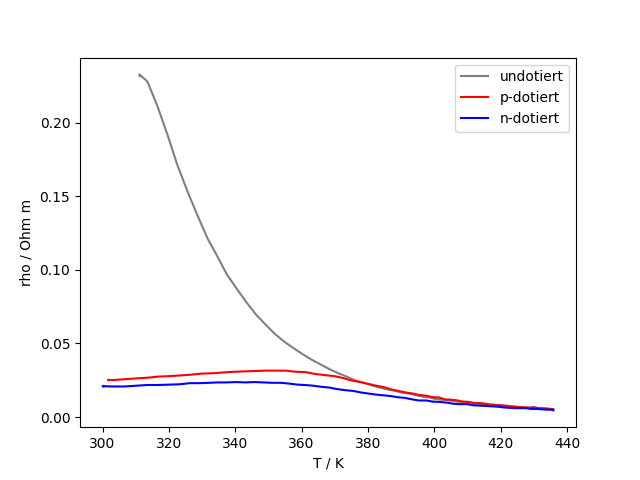
\includegraphics[scale=1.]{widerstand.png}
\caption{Widerstand der Germanium-Kristalle abhängig von deren Temperatur.}
\label{fig:leitfaehigkeit}
\end{figure}



Der Bandabstand von Germanium wird nun anhand des undotierten Kristalls bestimmt. Da der Zusammenhang zwischen Temperatur, Leitfähigkeit und Bandabstand durch die Gleichung
\begin{align*}
\sigma = \sigma_0 \cdot \exp\left(- \dfrac{E_G}{2\cdot k_B\cdot T}\right)
\end{align*}
bestimmt ist, kann man nun den Bandabstand durch Regression bestimmen. Dazu gilt
\begin{align*}
\log\left(\frac{\sigma}{\sigma_0}\right) = -\frac{E_G}{2\cdot k_B \cdot T }
\end{align*}
Wegen den Logarithmus-Regeln ist $\sigma_0$ vernachlässigbar (Achenabschnitt). Es ist nur die Steigung relevant. Es gilt also
\begin{align*}
\log(\sigma) = - \frac{E_G}{2\cdot k_B} \cdot \frac{1}{T}
\end{align*}
Invertiert man die Temperatur, so erhält man eine Geradengleichung
\begin{align*}
\log(\sigma) = - \frac{E_G}{2\cdot k_B} \cdot T
\end{align*}
Diese ist in Abbildung~\ref{fig:regression} dargestellt und zeigt tatsächlich eine Gerade. Durch lineare Regression erhält man die Steigung $k=-\dfrac{E_G}{2\cdot k_B}$ wobei $k$ die Boltzmann-Konstante ist.


\begin{figure}[H]
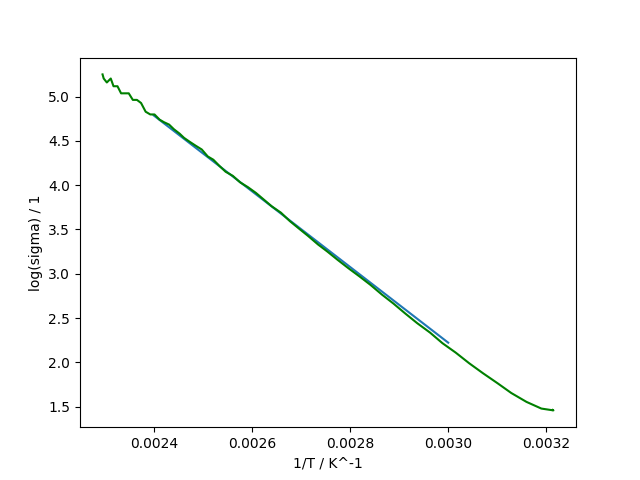
\includegraphics[scale=1.]{regression.png}
\caption{Regressionsgerade zur Berechnung des Bandabstandes.}
\label{fig:regression}
\end{figure}



Die Regression in Grafik~\ref{fig:regression} ergibt
\begin{align*}
k &= -4273.76~\text{K}^{-1}
\end{align*}
Daraus ergibt sich ein Bandabstand von
\begin{align*}
E_G &= -2\cdot k_B \cdot k = 0.74~\text{eV}
\end{align*}


\section{Diskussion}

Als Literaturwert für den Bandabstand wurde z.B. auf \cite{wikipedia} 0.67~eV angegeben. Dieser Wert passt von der Größenordnung und liegt auch innerhalb der entsprechenden Unsicherheit.

Für die Messung hätte man die Intervalle kleiner als 2 Sekunden wählen können. Dadurch hätte man bei der Leitfähigkeit glattere Kurven erhalten.

Eine weitere Möglichkeit zur Optimierung der Genauigkeit des Bandabstandes wäre die Messung bei mehreren Querströmen. 




\section{Zusammenfassung}

Es wurde dsa Leitverhalten von dotiertem und undotierten Germanium beschrieben. Für den Bandabstand von Germanium wurde der Wert
\begin{align*}
E_G &= (0.74 \pm 0.07) ~\text{eV}
\end{align*}
erhalten, was durchaus plausibel ist.


\begin{thebibliography}{9}
\bibitem{moodle} G. Koller: Skript zum Bandabstand von Germanium aus dem Moodle der Karl-Franzens Universität, Institut für Physik, 22.05.2021.
\bibitem{messmethoden}  R. Dämon: Einführung in die physikalischen Messmethoden, Graz 2016.
\bibitem{demtroeder} W. Demtröder: \emph{Experimentalphysik 2 - Elektrizität  und Optik}, 7. Auflage, 2017.
\bibitem{python} Python-Skript zur Berechnung der Daten, zur Visualisierung und zum Generieren von \LaTeX-Code für diesen Bericht.
\bibitem{wikipedia} \url{https://de.wikipedia.org/wiki/Halbleiter_mit_breitem_Bandabstand}, 22.05.2021.
\end{thebibliography}


\newpage 
%\appendix
%\section{Python Skript}



\definecolor{commentgreen}{RGB}{2,112,10}
\definecolor{eminence}{RGB}{108,48,130}
\definecolor{weborange}{RGB}{255,165,0}
\definecolor{frenchplum}{RGB}{129,20,83}

\lstdefinelanguage{python}{
    morekeywords={def, for, range, abs, return},
    otherkeywords={<-,->, |>, \%\{, \}, \{, \, (, )},
    sensitive=true,
    morecomment=[l]{\#},
    morecomment=[n]{/*}{*/},
    morecomment=[s][\color{purple}]{:}{\ },
    morestring=[s][\color{orange}]"",
    commentstyle=\color{commentgreen},
    keywordstyle=\color{eminence},
    stringstyle=\color{red},
	basicstyle=\ttfamily,
	breaklines,
	showstringspaces=false,
	frame=tb
}
%\lstinputlisting[language=Python,captionpos=b, label=lst:test,caption={Auswertung}]{script.py}

%\lstinputlisting[language=Python,captionpos=b, label=lst:test,caption={Bessel Auswertung}]{generate_numbers_bessel.py}



\end{document}